% Created by tikzDevice version 0.7.0 on 2014-12-04 12:50:36
% !TEX encoding = UTF-8 Unicode
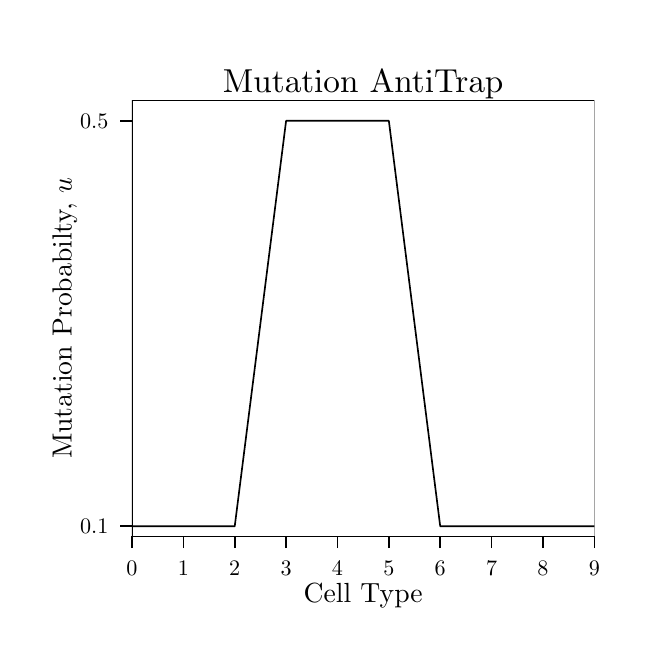
\begin{tikzpicture}[x=1pt,y=1pt]
\definecolor[named]{fillColor}{rgb}{1.00,1.00,1.00}
\path[use as bounding box,fill=fillColor,fill opacity=0.00] (0,0) rectangle (216.81,216.81);
\begin{scope}
\path[clip] (  0.00,  0.00) rectangle (216.81,216.81);
\definecolor[named]{drawColor}{rgb}{1.00,1.00,1.00}
\definecolor[named]{fillColor}{rgb}{1.00,1.00,1.00}

\path[draw=drawColor,line width= 0.6pt,line join=round,line cap=round,fill=fillColor] (  0.00,  0.00) rectangle (216.81,216.81);
\end{scope}
\begin{scope}
\path[clip] ( 37.69, 32.98) rectangle (204.76,190.48);
\definecolor[named]{fillColor}{rgb}{1.00,1.00,1.00}

\path[fill=fillColor] ( 37.69, 32.98) rectangle (204.76,190.48);
\definecolor[named]{drawColor}{rgb}{0.00,0.00,0.00}

\path[draw=drawColor,line width= 0.6pt,line join=round] ( 37.69, 36.64) --
	( 56.25, 36.64) --
	( 74.82, 36.64) --
	( 93.38,183.15) --
	(111.94,183.15) --
	(130.51,183.15) --
	(149.07, 36.64) --
	(167.64, 36.64) --
	(186.20, 36.64) --
	(204.76, 36.64);

\path[draw=drawColor,line width= 0.6pt,line join=round,line cap=round] ( 37.69, 32.98) rectangle (204.76,190.48);
\end{scope}
\begin{scope}
\path[clip] (  0.00,  0.00) rectangle (216.81,216.81);
\definecolor[named]{drawColor}{rgb}{0.00,0.00,0.00}

\node[text=drawColor,anchor=base east,inner sep=0pt, outer sep=0pt, scale=  0.80] at ( 29.15, 33.89) {0.1};

\node[text=drawColor,anchor=base east,inner sep=0pt, outer sep=0pt, scale=  0.80] at ( 29.15,180.40) {0.5};
\end{scope}
\begin{scope}
\path[clip] (  0.00,  0.00) rectangle (216.81,216.81);
\definecolor[named]{drawColor}{rgb}{0.00,0.00,0.00}

\path[draw=drawColor,line width= 0.6pt,line join=round] ( 33.42, 36.64) --
	( 37.69, 36.64);

\path[draw=drawColor,line width= 0.6pt,line join=round] ( 33.42,183.15) --
	( 37.69,183.15);
\end{scope}
\begin{scope}
\path[clip] (  0.00,  0.00) rectangle (216.81,216.81);
\definecolor[named]{drawColor}{rgb}{0.00,0.00,0.00}

\path[draw=drawColor,line width= 0.6pt,line join=round] ( 37.69, 28.71) --
	( 37.69, 32.98);

\path[draw=drawColor,line width= 0.6pt,line join=round] ( 56.25, 28.71) --
	( 56.25, 32.98);

\path[draw=drawColor,line width= 0.6pt,line join=round] ( 74.82, 28.71) --
	( 74.82, 32.98);

\path[draw=drawColor,line width= 0.6pt,line join=round] ( 93.38, 28.71) --
	( 93.38, 32.98);

\path[draw=drawColor,line width= 0.6pt,line join=round] (111.94, 28.71) --
	(111.94, 32.98);

\path[draw=drawColor,line width= 0.6pt,line join=round] (130.51, 28.71) --
	(130.51, 32.98);

\path[draw=drawColor,line width= 0.6pt,line join=round] (149.07, 28.71) --
	(149.07, 32.98);

\path[draw=drawColor,line width= 0.6pt,line join=round] (167.64, 28.71) --
	(167.64, 32.98);

\path[draw=drawColor,line width= 0.6pt,line join=round] (186.20, 28.71) --
	(186.20, 32.98);

\path[draw=drawColor,line width= 0.6pt,line join=round] (204.76, 28.71) --
	(204.76, 32.98);
\end{scope}
\begin{scope}
\path[clip] (  0.00,  0.00) rectangle (216.81,216.81);
\definecolor[named]{drawColor}{rgb}{0.00,0.00,0.00}

\node[text=drawColor,anchor=base,inner sep=0pt, outer sep=0pt, scale=  0.80] at ( 37.69, 18.93) {0};

\node[text=drawColor,anchor=base,inner sep=0pt, outer sep=0pt, scale=  0.80] at ( 56.25, 18.93) {1};

\node[text=drawColor,anchor=base,inner sep=0pt, outer sep=0pt, scale=  0.80] at ( 74.82, 18.93) {2};

\node[text=drawColor,anchor=base,inner sep=0pt, outer sep=0pt, scale=  0.80] at ( 93.38, 18.93) {3};

\node[text=drawColor,anchor=base,inner sep=0pt, outer sep=0pt, scale=  0.80] at (111.94, 18.93) {4};

\node[text=drawColor,anchor=base,inner sep=0pt, outer sep=0pt, scale=  0.80] at (130.51, 18.93) {5};

\node[text=drawColor,anchor=base,inner sep=0pt, outer sep=0pt, scale=  0.80] at (149.07, 18.93) {6};

\node[text=drawColor,anchor=base,inner sep=0pt, outer sep=0pt, scale=  0.80] at (167.64, 18.93) {7};

\node[text=drawColor,anchor=base,inner sep=0pt, outer sep=0pt, scale=  0.80] at (186.20, 18.93) {8};

\node[text=drawColor,anchor=base,inner sep=0pt, outer sep=0pt, scale=  0.80] at (204.76, 18.93) {9};
\end{scope}
\begin{scope}
\path[clip] (  0.00,  0.00) rectangle (216.81,216.81);
\definecolor[named]{drawColor}{rgb}{0.00,0.00,0.00}

\node[text=drawColor,anchor=base,inner sep=0pt, outer sep=0pt, scale=  1.00] at (121.23,  9.03) {Cell Type};
\end{scope}
\begin{scope}
\path[clip] (  0.00,  0.00) rectangle (216.81,216.81);
\definecolor[named]{drawColor}{rgb}{0.00,0.00,0.00}

\node[text=drawColor,rotate= 90.00,anchor=base,inner sep=0pt, outer sep=0pt, scale=  1.00] at ( 15.92,111.73) {Mutation Probabilty, $u$};
\end{scope}
\begin{scope}
\path[clip] (  0.00,  0.00) rectangle (216.81,216.81);
\definecolor[named]{drawColor}{rgb}{0.00,0.00,0.00}

\node[text=drawColor,anchor=base,inner sep=0pt, outer sep=0pt, scale=  1.20] at (121.23,193.49) {Mutation AntiTrap};
\end{scope}
\end{tikzpicture}
